\subsection{Endoplasmic Reticulum}
    \subsubsection{Preprocessing}
        

\begin{algorithm}
    \caption{Fluorescence segmentation}\label{alg:global-thresholding}
    \begin{algorithmic}
    \item 1. Normalize image
    \item 2. Apply global \textit{threshold\_mean} to receive initial mask.
    \item 3. Zero out pixels outside the mask
    \item 4. Apply local thresholding.  
    \item 5. Apply \textit{fill\_holes} transformation.
    \item 6. Morphological opening from OpenCV and Gaussian blur.
    \item 7. Run \textit{findContours} from OpenCV in order to obtain separate regions and filter out too small regions.
    \end{algorithmic}
\end{algorithm}    

Segmentation steps are also illustrated in Figure \begin{figure}[H]
    \centering
    \setkeys{Gin}{width=\linewidth}
    \centering
        \begin{tabularx}{\textwidth}{YYYYYYY}
            \textbf{1} &
            \textbf{2} &
            \textbf{3} &
            \textbf{4} &
            \textbf{5} &
            \textbf{6} &
            \textbf{7} \\
            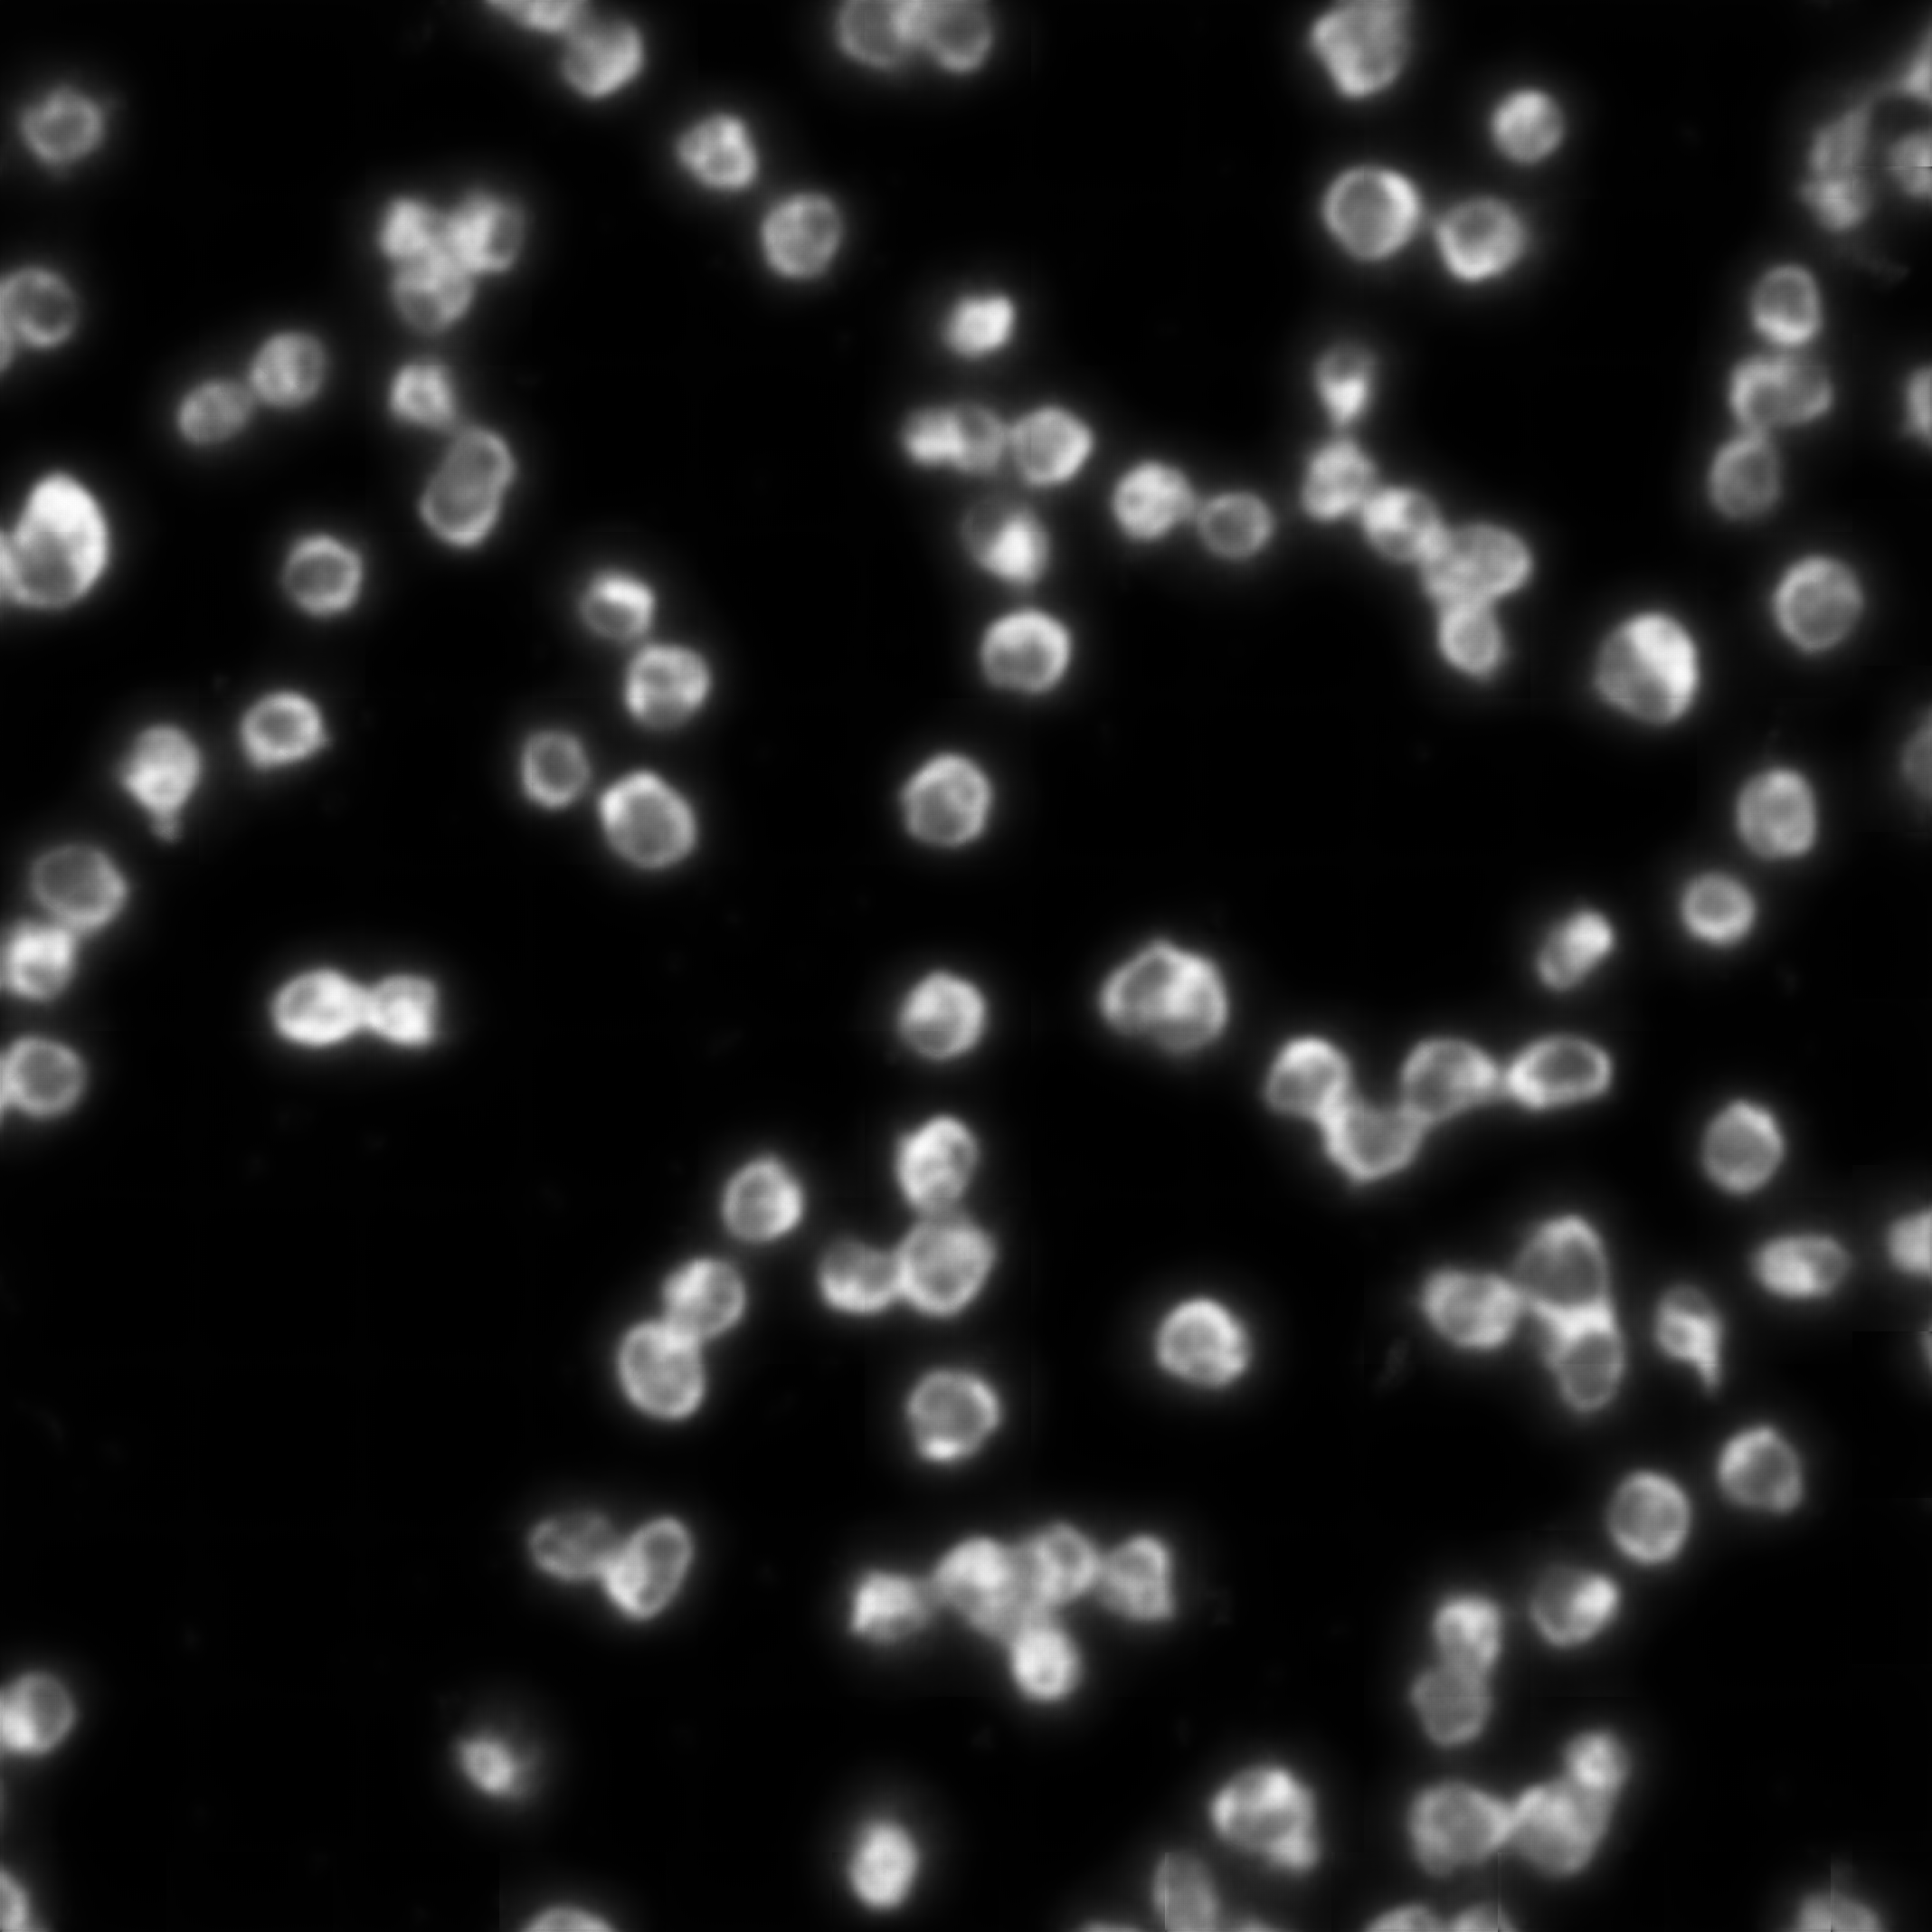
\includegraphics{bilder/ER/segmentation/pp_1.png} & 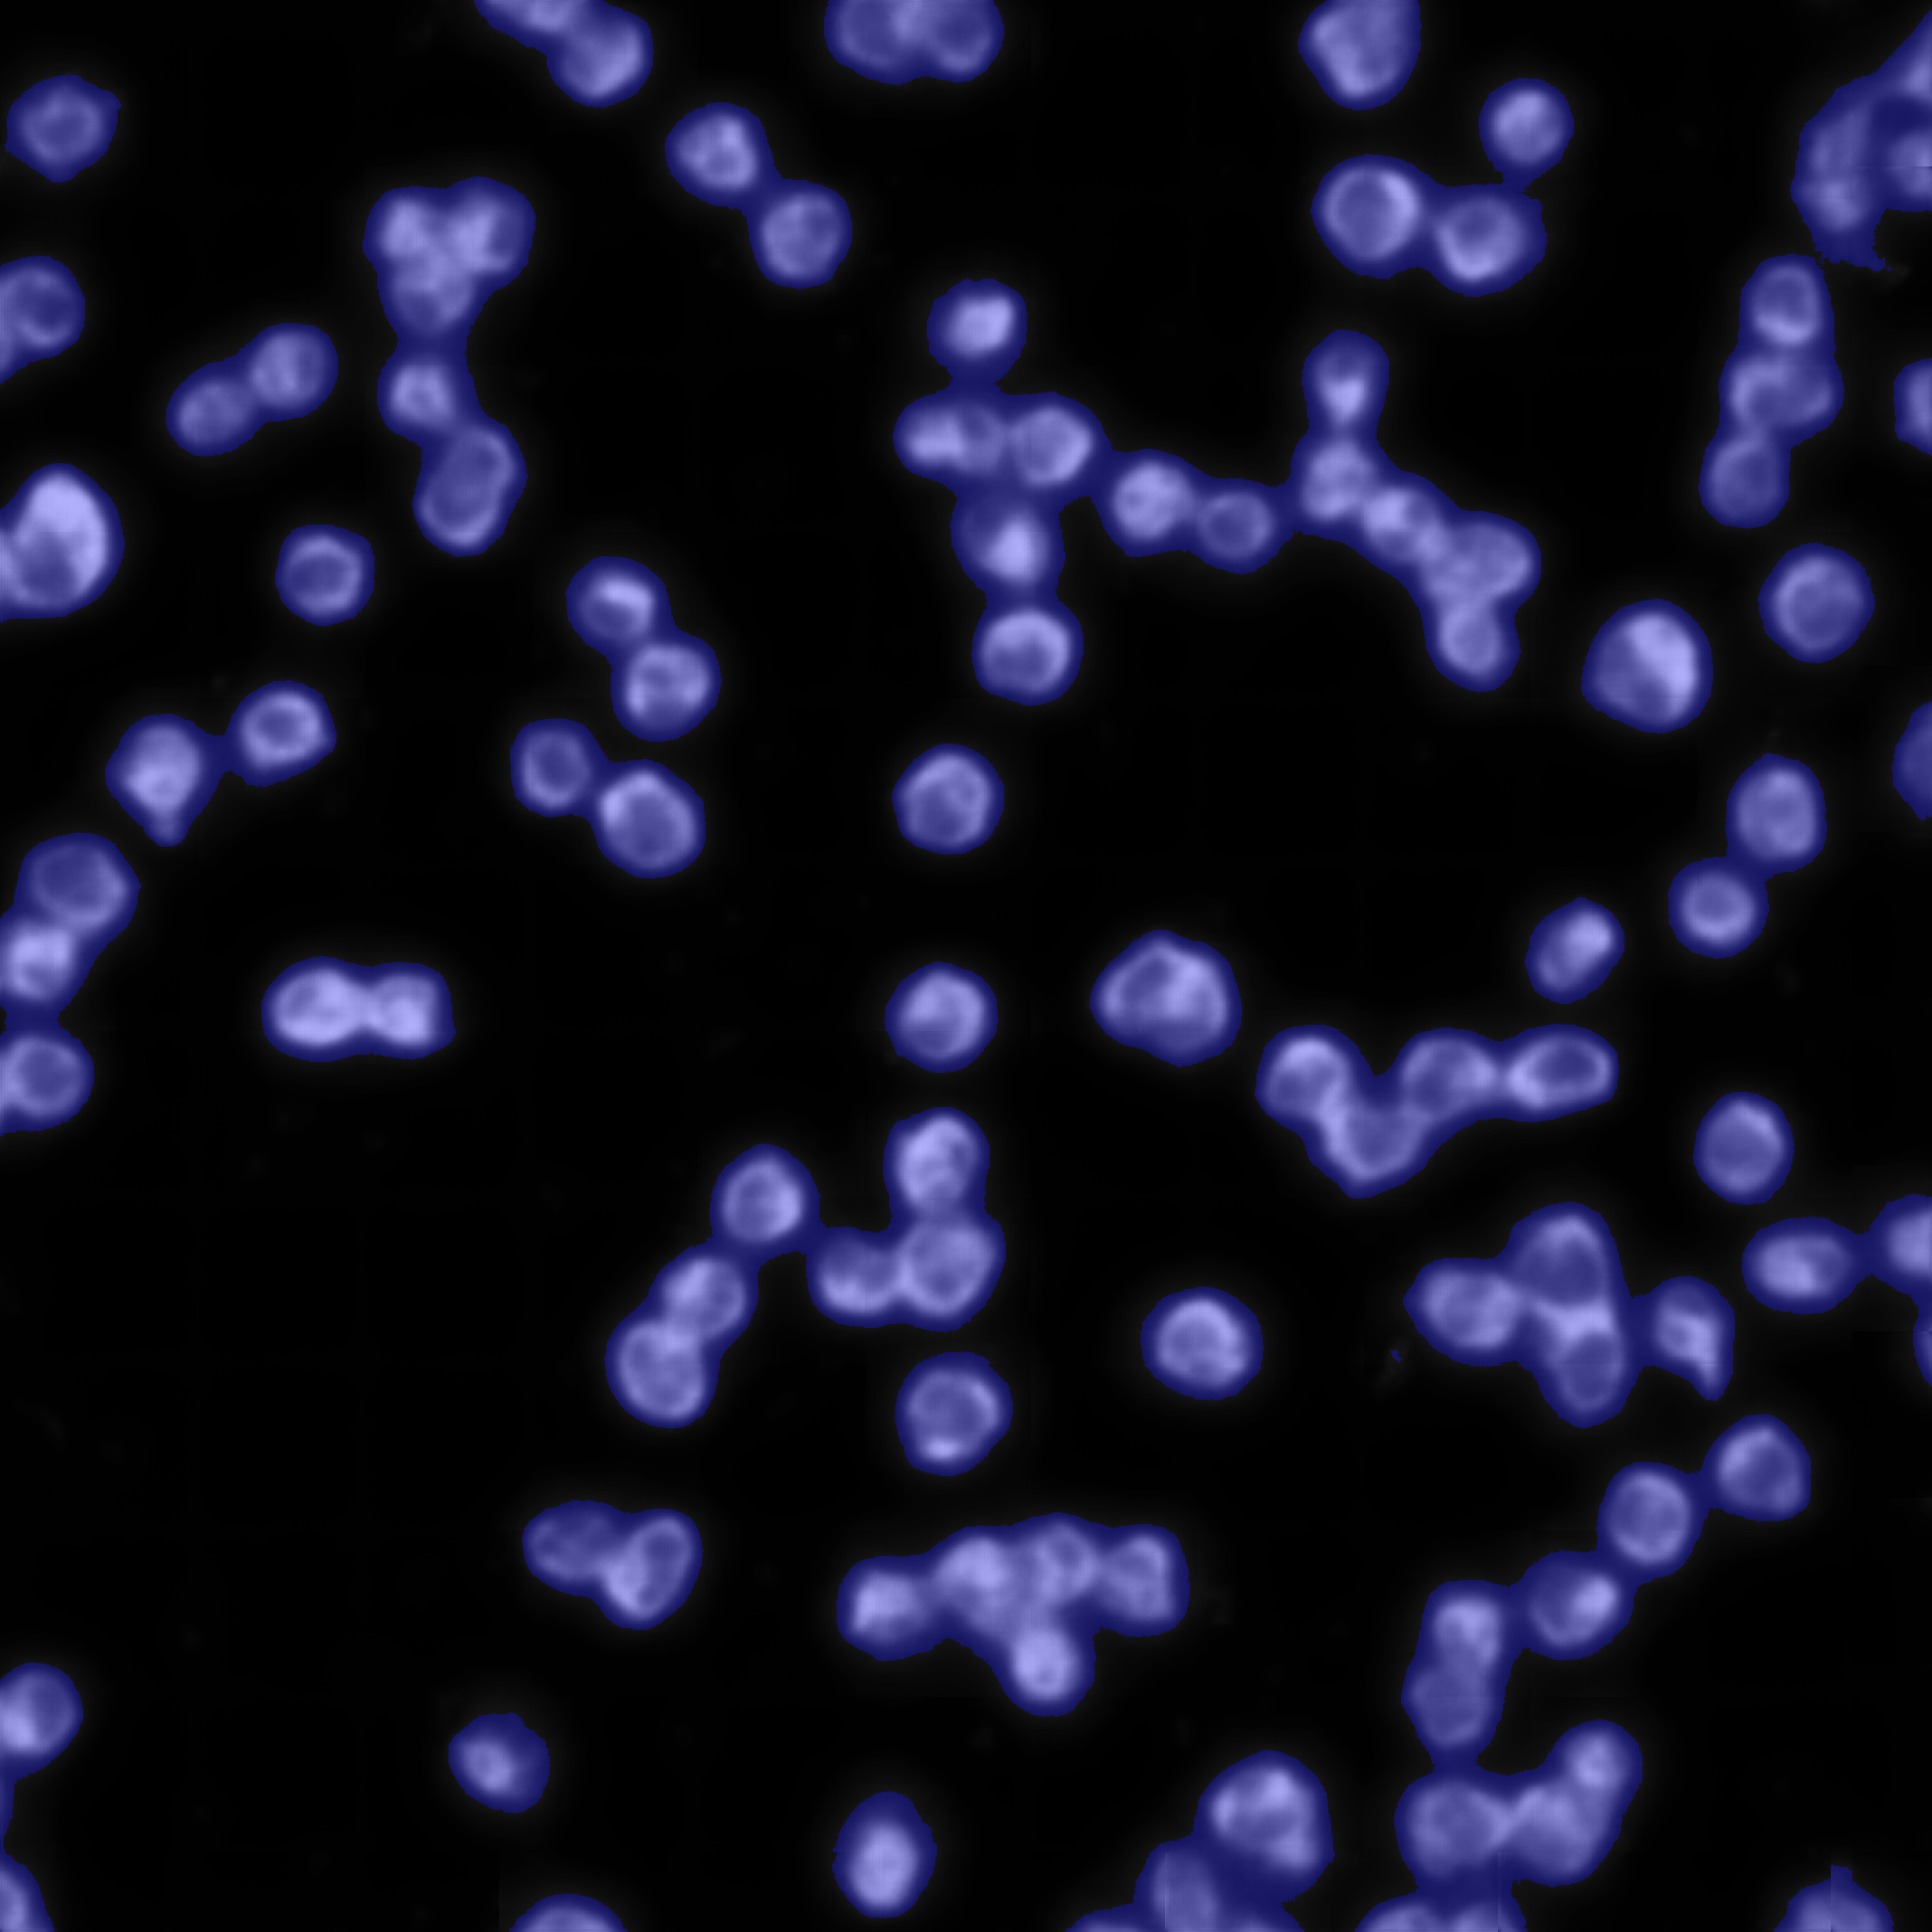
\includegraphics{bilder/ER/segmentation/pp_2.png} &
            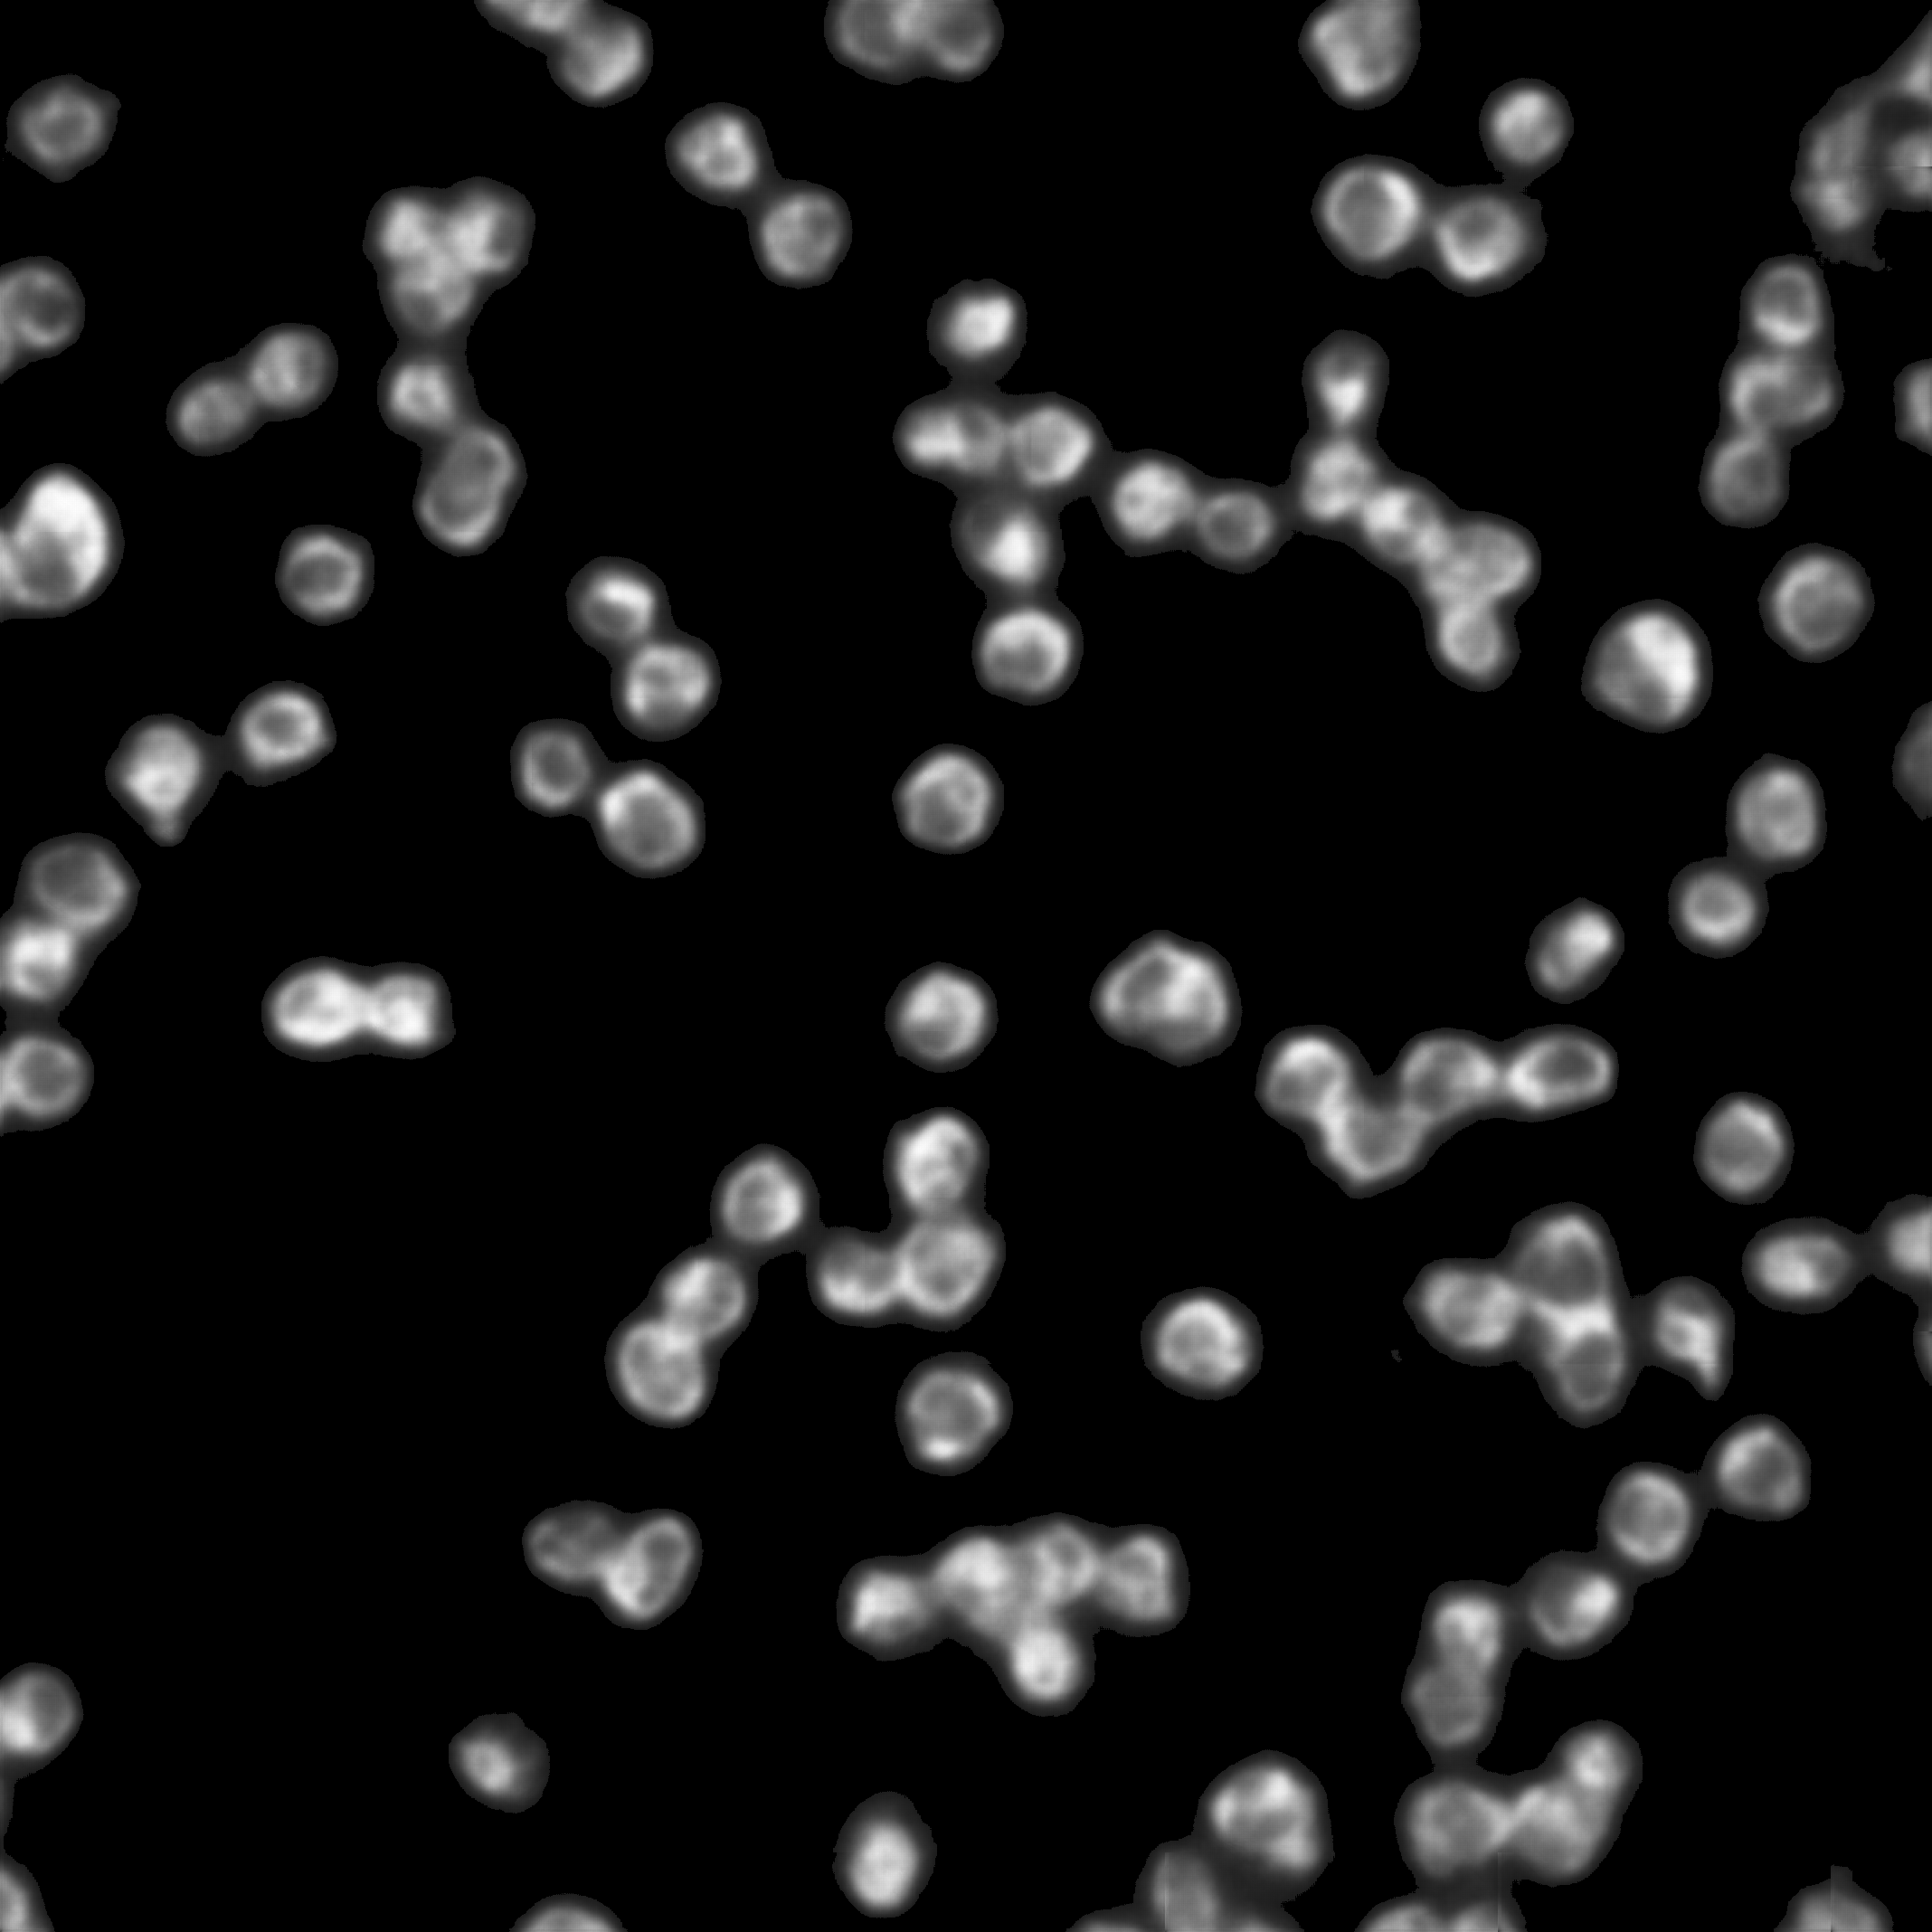
\includegraphics{bilder/ER/segmentation/pp_3.png} &
            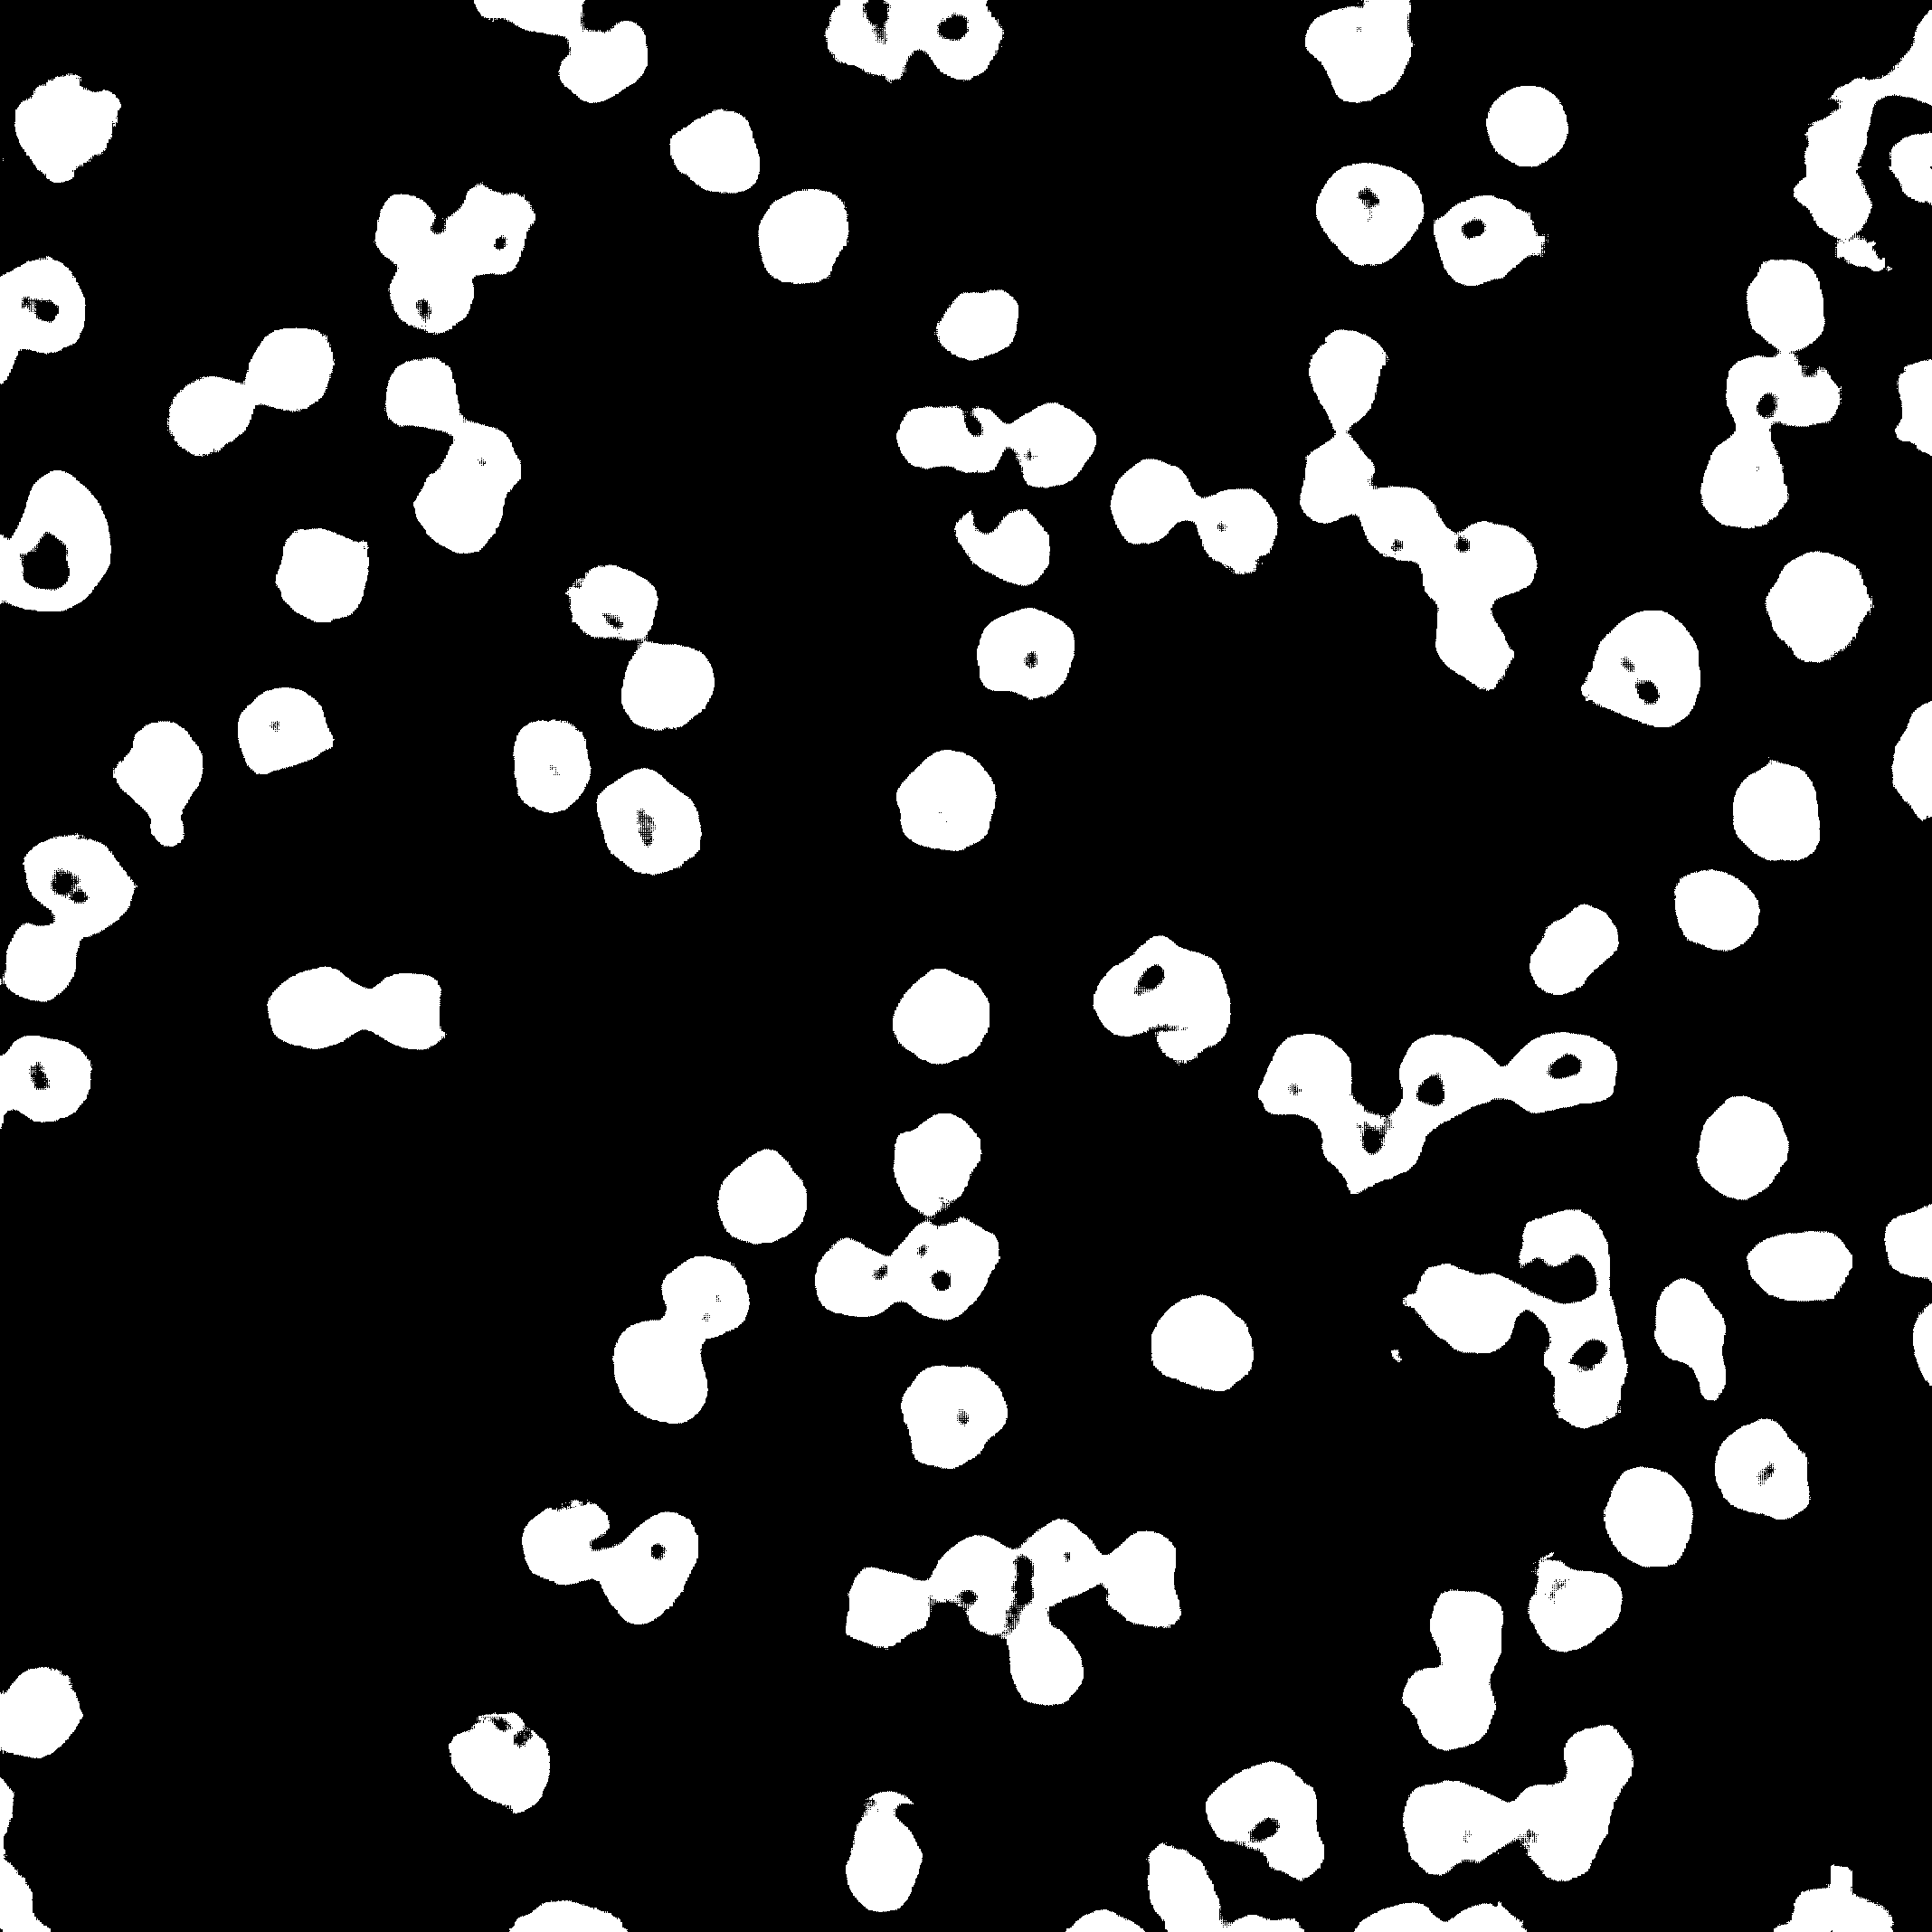
\includegraphics{bilder/ER/segmentation/pp_4.png} &
            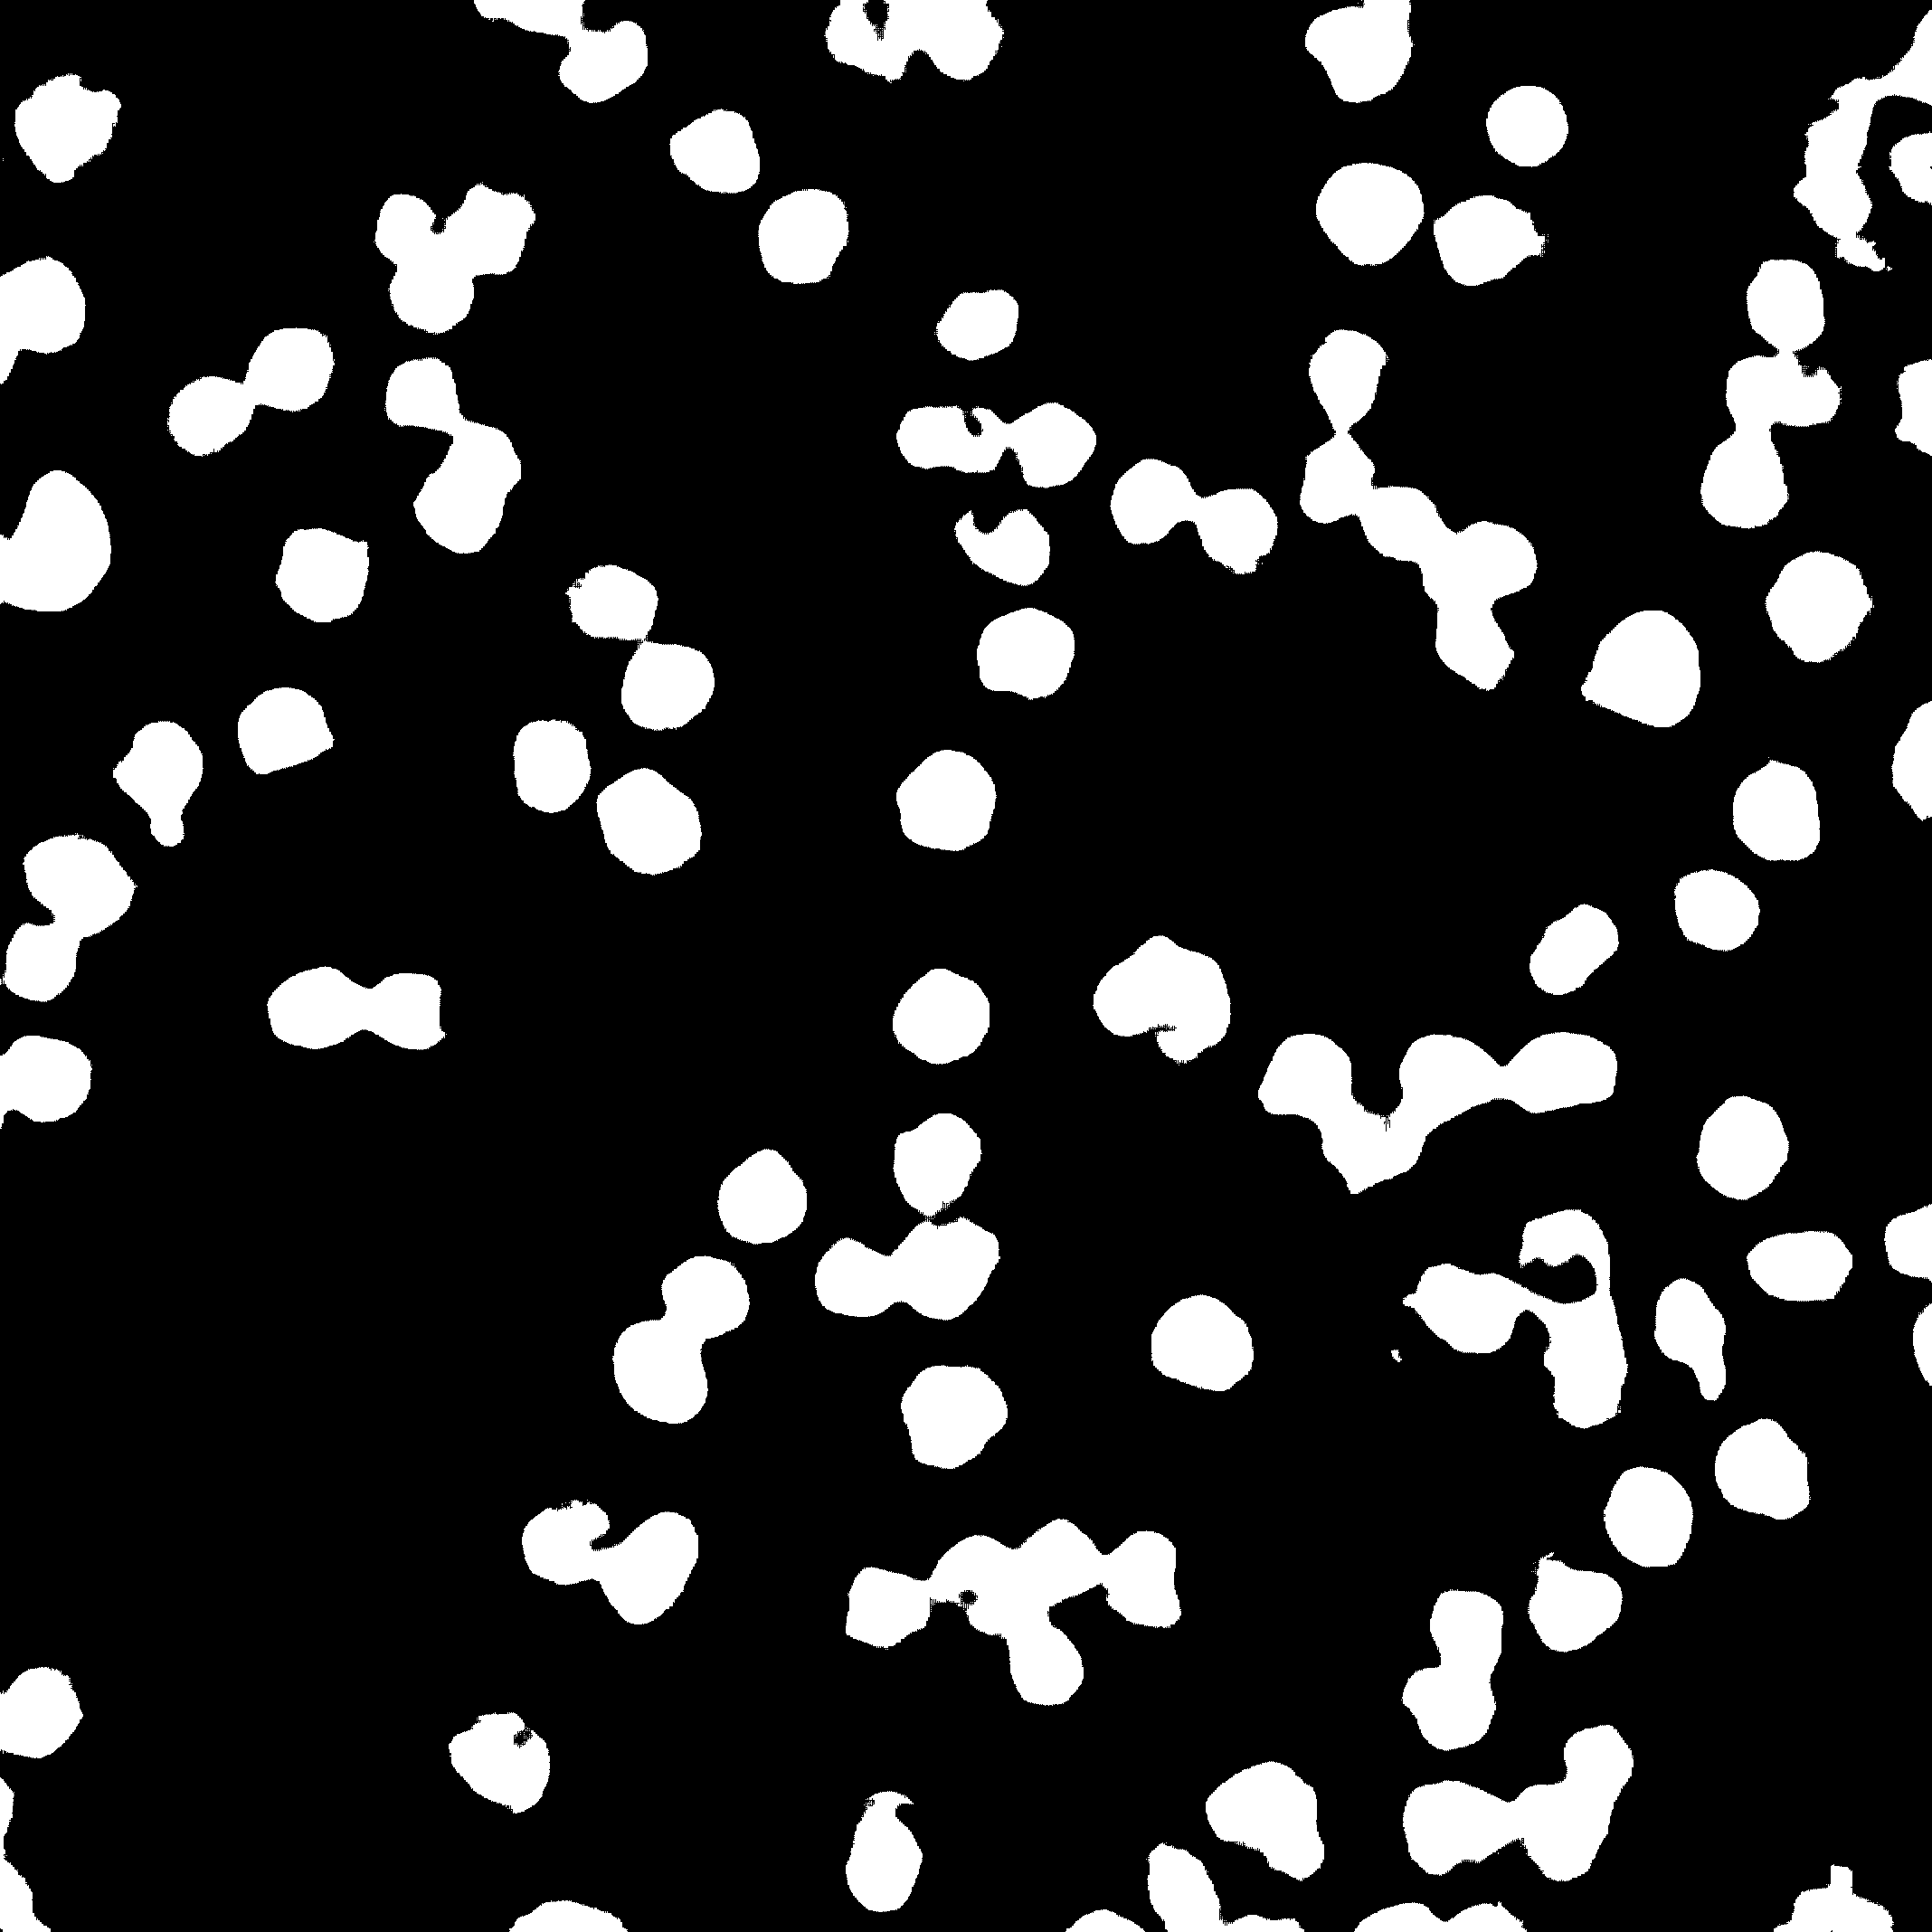
\includegraphics{bilder/ER/segmentation/pp_5.png} &
            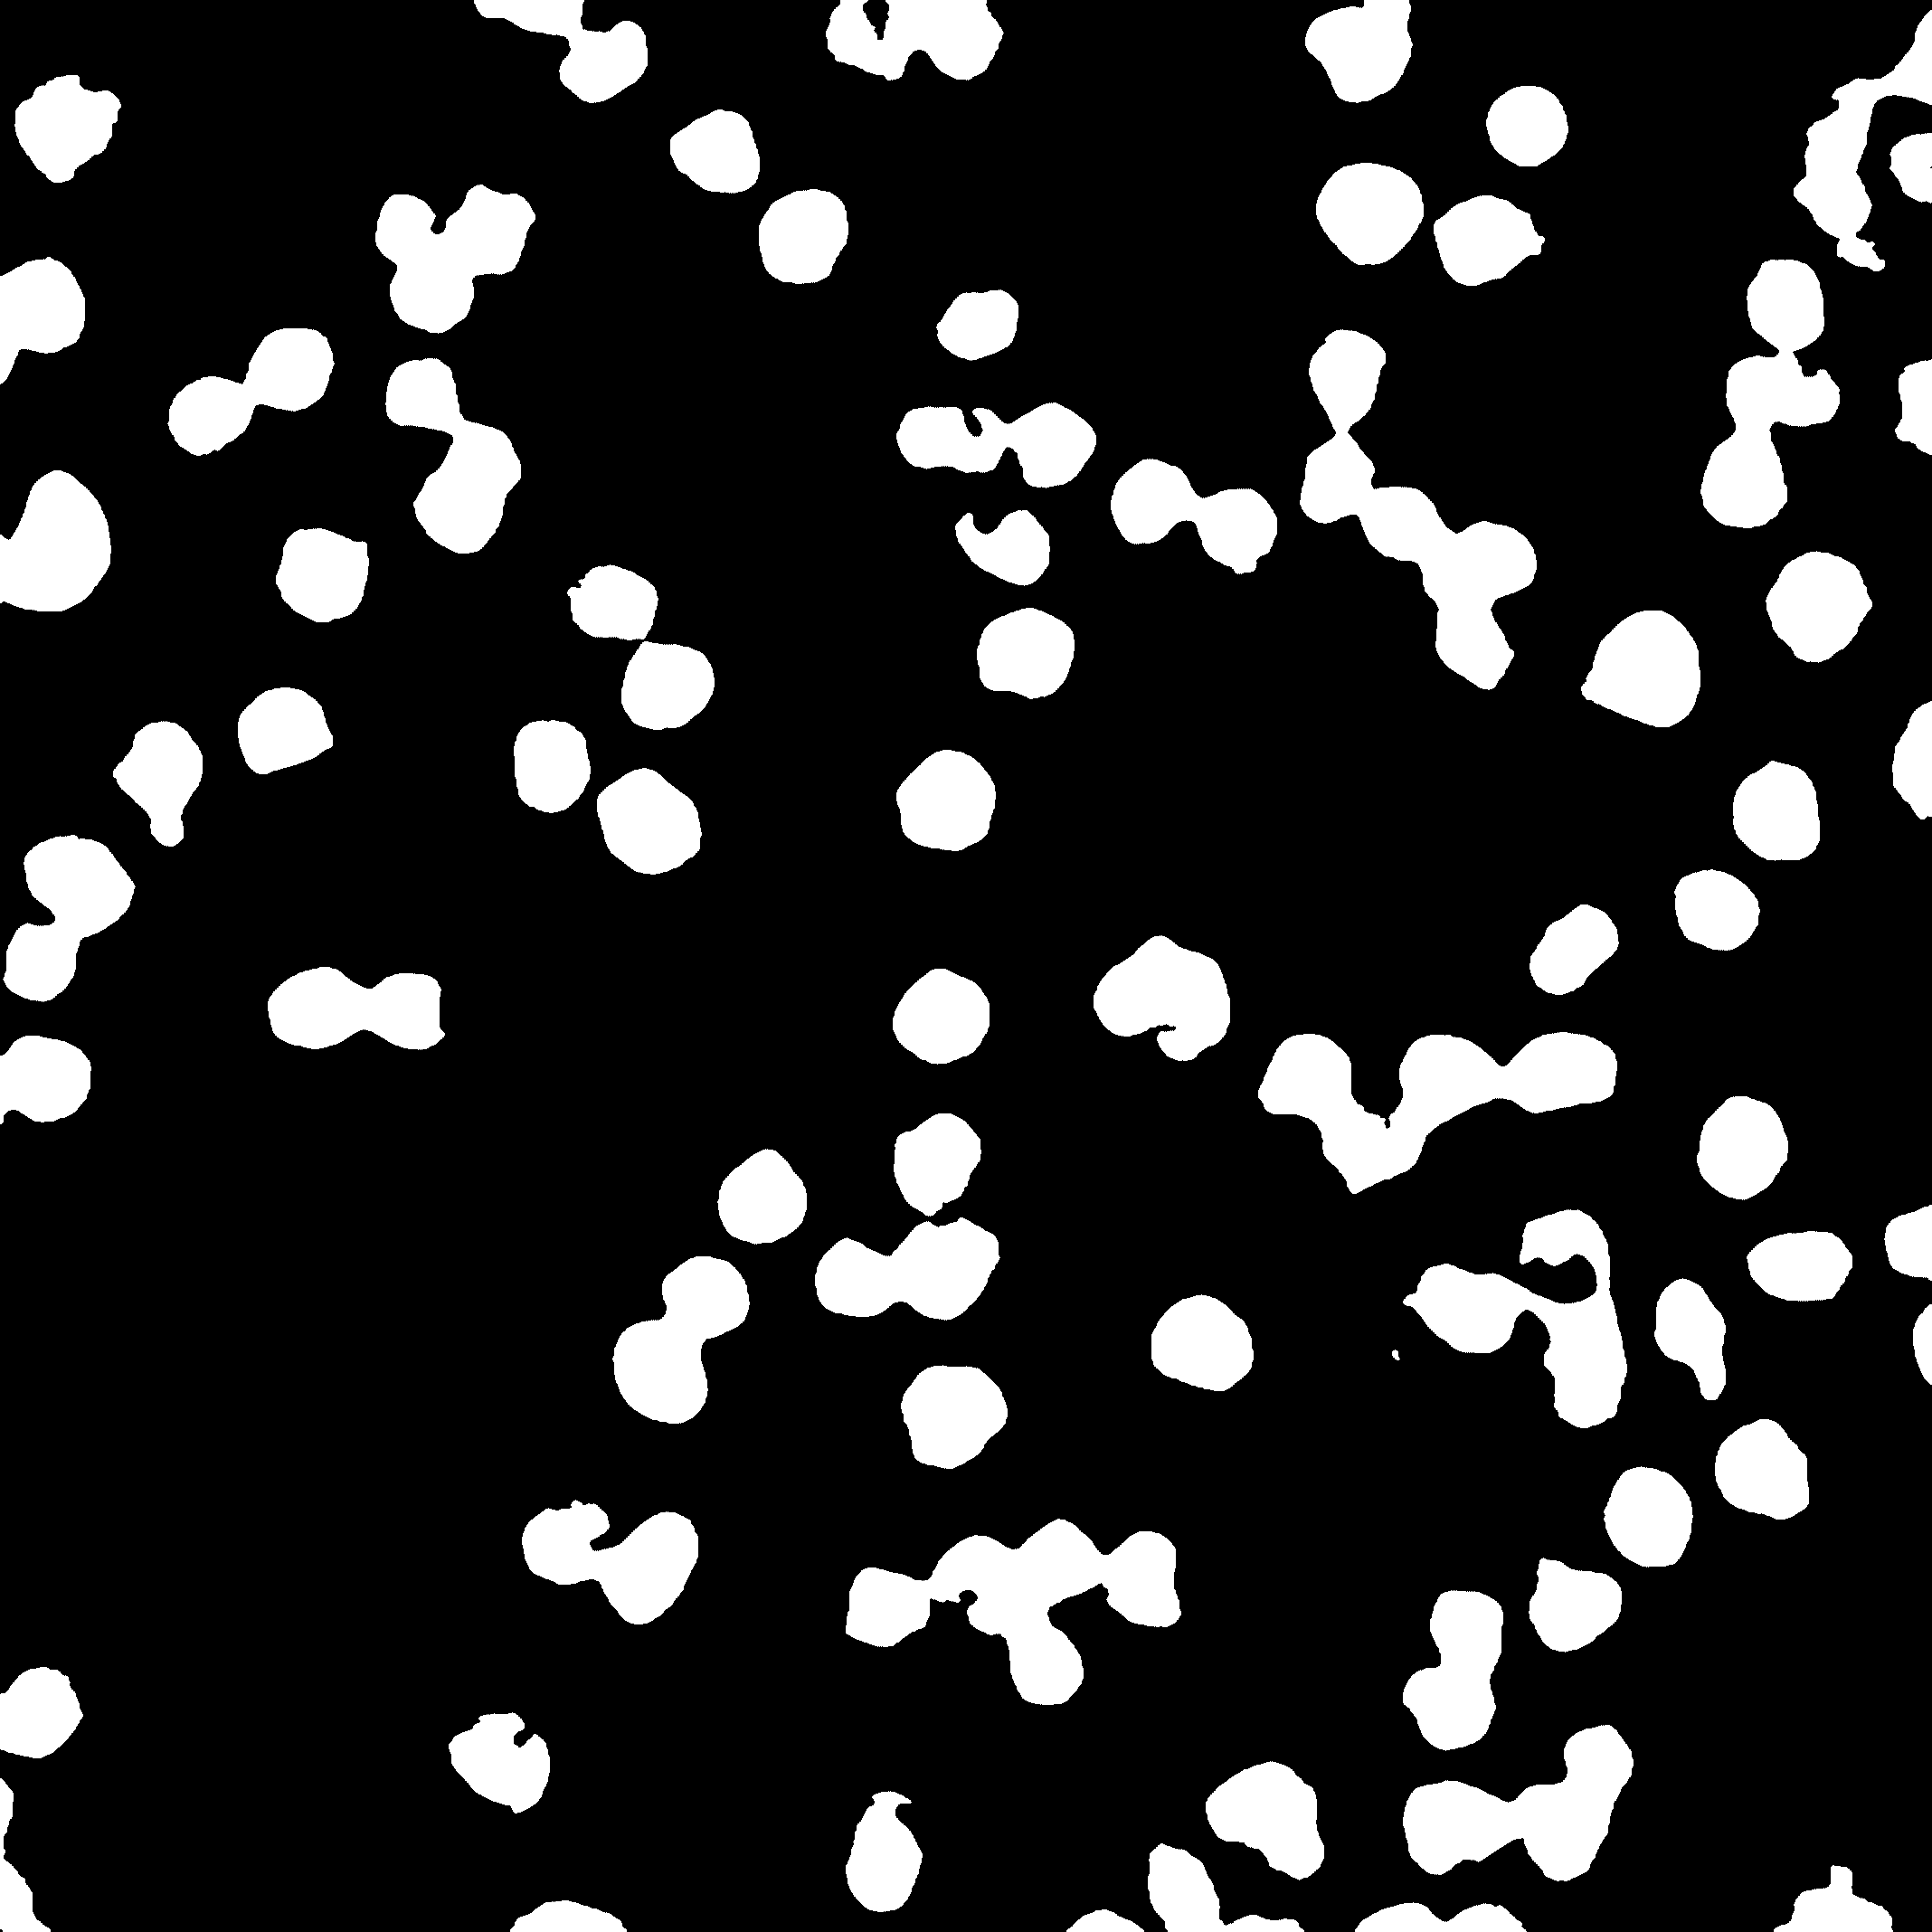
\includegraphics{bilder/ER/segmentation/pp_6.png} &
            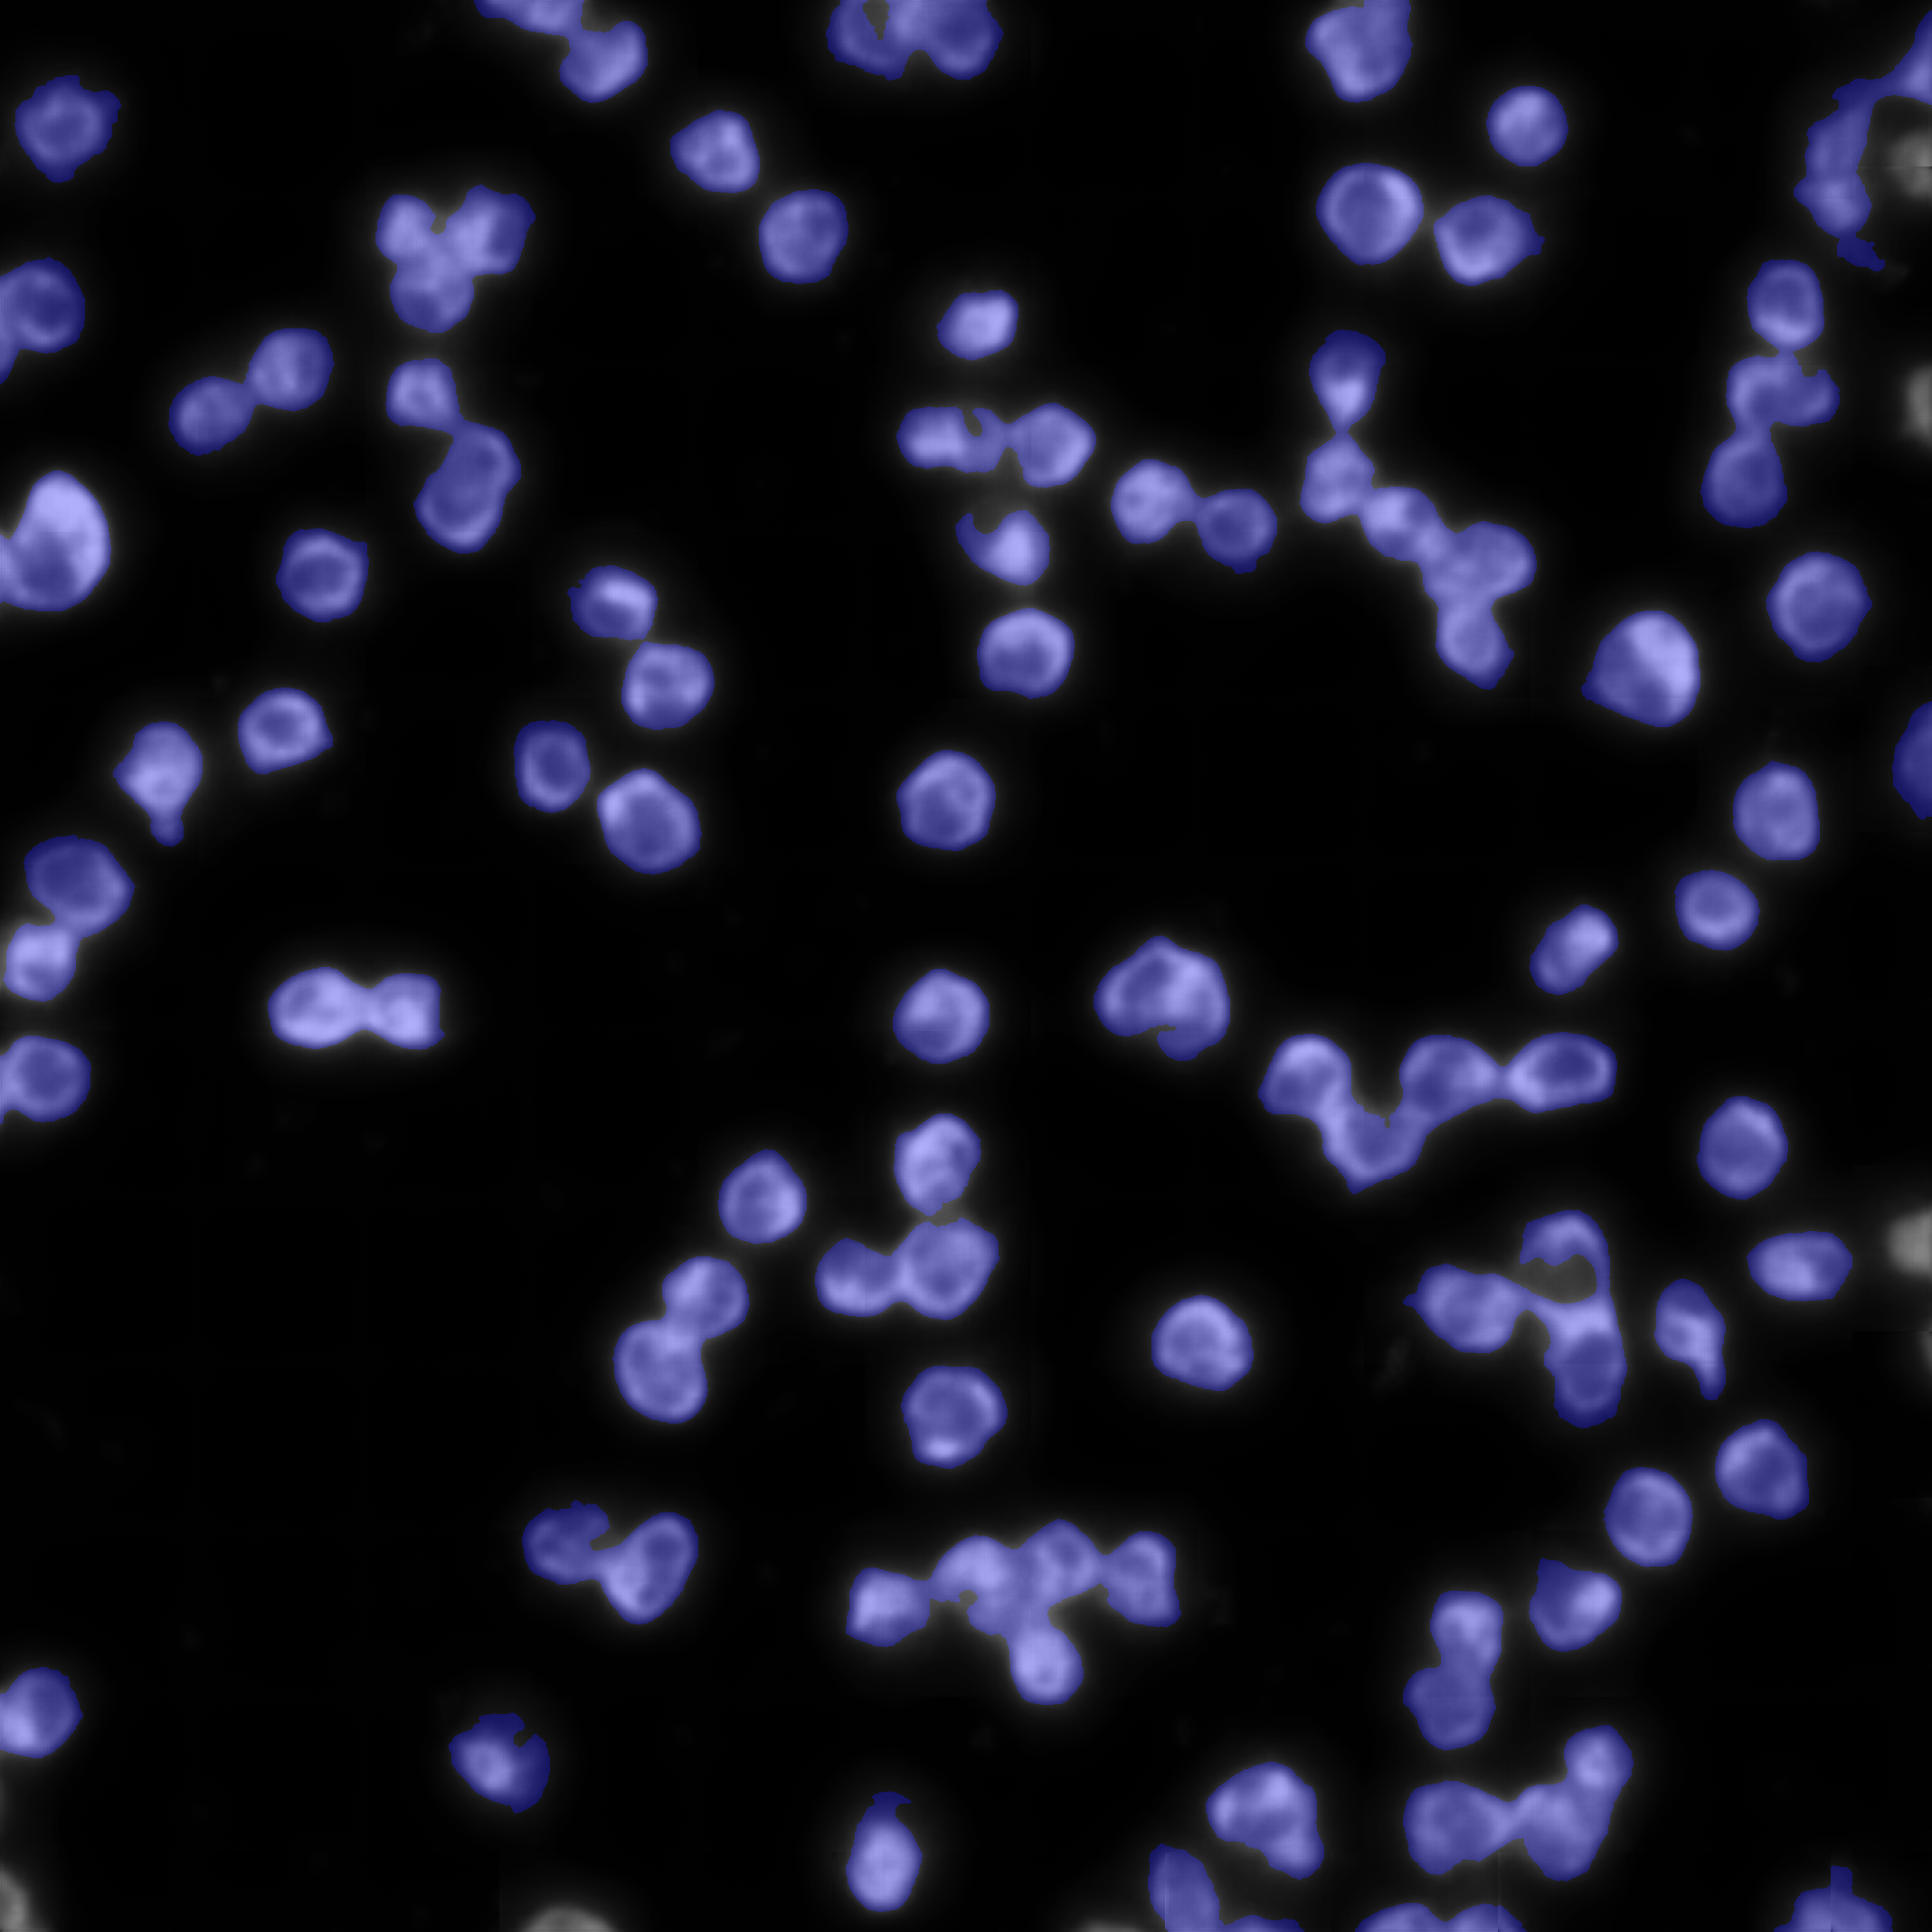
\includegraphics{bilder/ER/segmentation/pp_7.png} 
        \end{tabularx}
    \caption{ER prediction}
    \label{fig:er-prediction}
\end{figure}
    \subsubsection{Training and predictions}
        During the training with PCC loss the model has successfully converged already after 35 epochs, however a clear overfit was encountered (see Figure \ref{fig:er-overfit} (left)) with the best PCC loss before the overfit being $0.0713$. Overfitting happens due to the lack of data, as for ER case there were much fewer samples than for nuclei for example (see Table \ref{table:data}). Even though one could use early-stopping approach and simply choose an earlier epoch before overfit, the better approach would be to use regularization methods described in section \ref{section:regularization}. Additional regularization in terms of data augmentations was introduced. The new learning curve is shown in Figure \ref{fig:er-overfit} (middle). Overfit happens now much later (after $120$ epochs) and PCC loss improves to $0.0701$. Introducing a stronger regularization with the use of weight decay in adadelta optimizer and dropout layers with a dropout rate of $0.1$ (see Figure \ref{fig:er-overfit} (right)) reduces the overfit completely, however at the same time increases the loss to $0.099$.
\begin{figure}[H]
	\begin{center}
		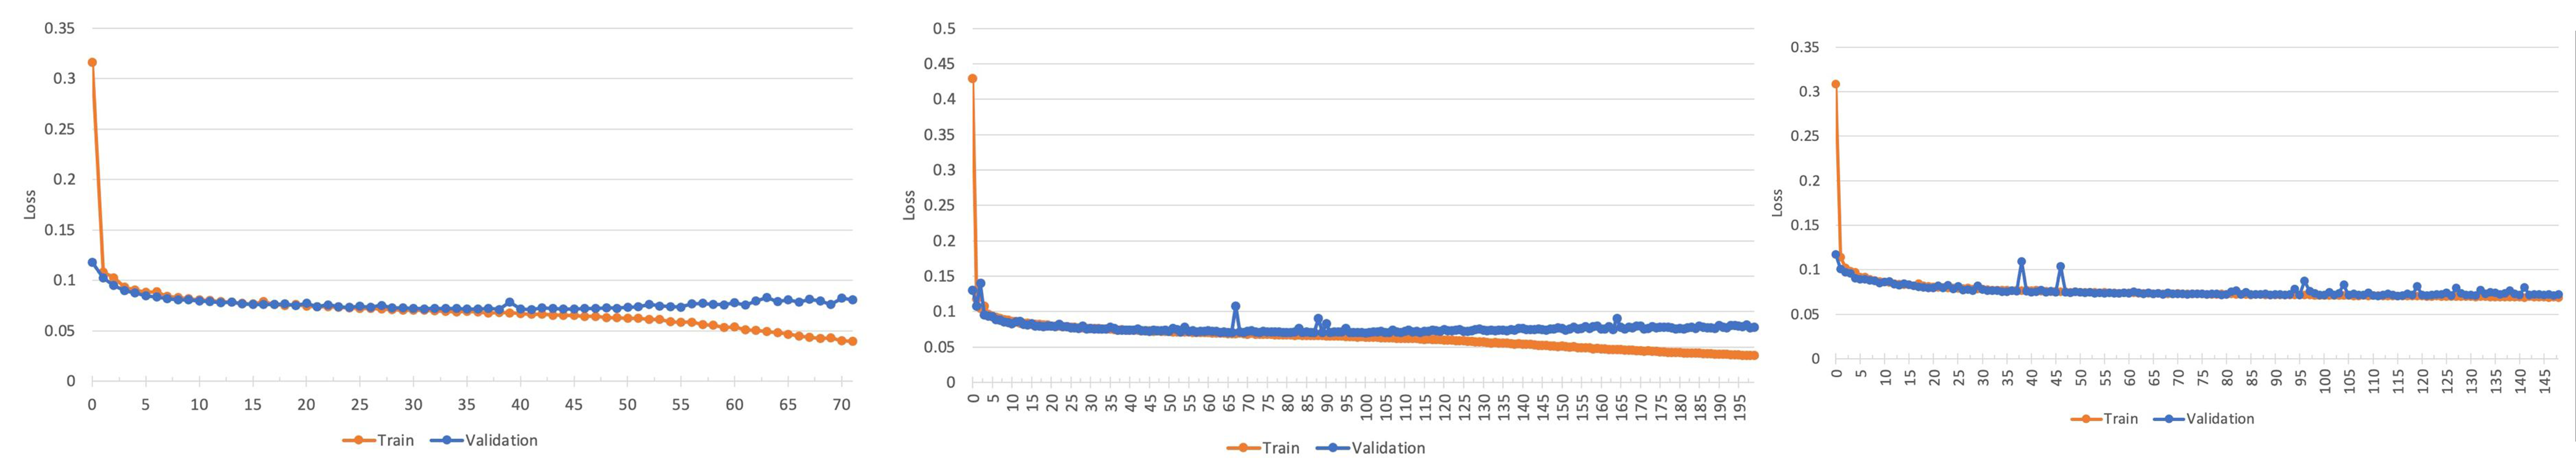
\includegraphics[width=\linewidth]{bilder/ER/segmentation/reg-not-reg.png}
		\caption{Default model (left), slightly regularized model(middle), strongly regularized model (right)}\label{fig:er-overfit}
	\end{center}
\end{figure}

Although the validation loss seem to be higher in comparison to $0.0701$, in this case the growths were not explained by the difference between the validation sets, where the loss was measured on. PCC losses on the same validation set for both were $0.0701$ and $0.0742$. It might have been the case that the regularization was too strong. In this case it would be better to use early-stopping approach with the epoch that has the lowest loss.
    \subsubsection{Combination of nuclei and actin predictions}
        Now having two models for the predictions of two organelles: nuclei and ER, it is interesting to visualize the predictions together (see Figure \ref{fig:er-combined}). It is clear from the image that ER indeed is located around the nucleus. As one can see, there is a great advantage in the used of \textit{in silico} fluroescence labeling especially for the cases where several cell targets have to be ananlysed. Instead of a expesive and time-consuming procedure for staining several targets at the same time they can be predicted based on one DIC image only.
\begin{figure}[htb]
    \centering
    \setkeys{Gin}{width=\linewidth}
    \centering
        \begin{tabularx}{\textwidth}{YYYY}
            (a)  \textbf{Ground truth} &
            (b)  \textbf{Prediction} &
            (c)  \textbf{Prediction + nuclei} \\
            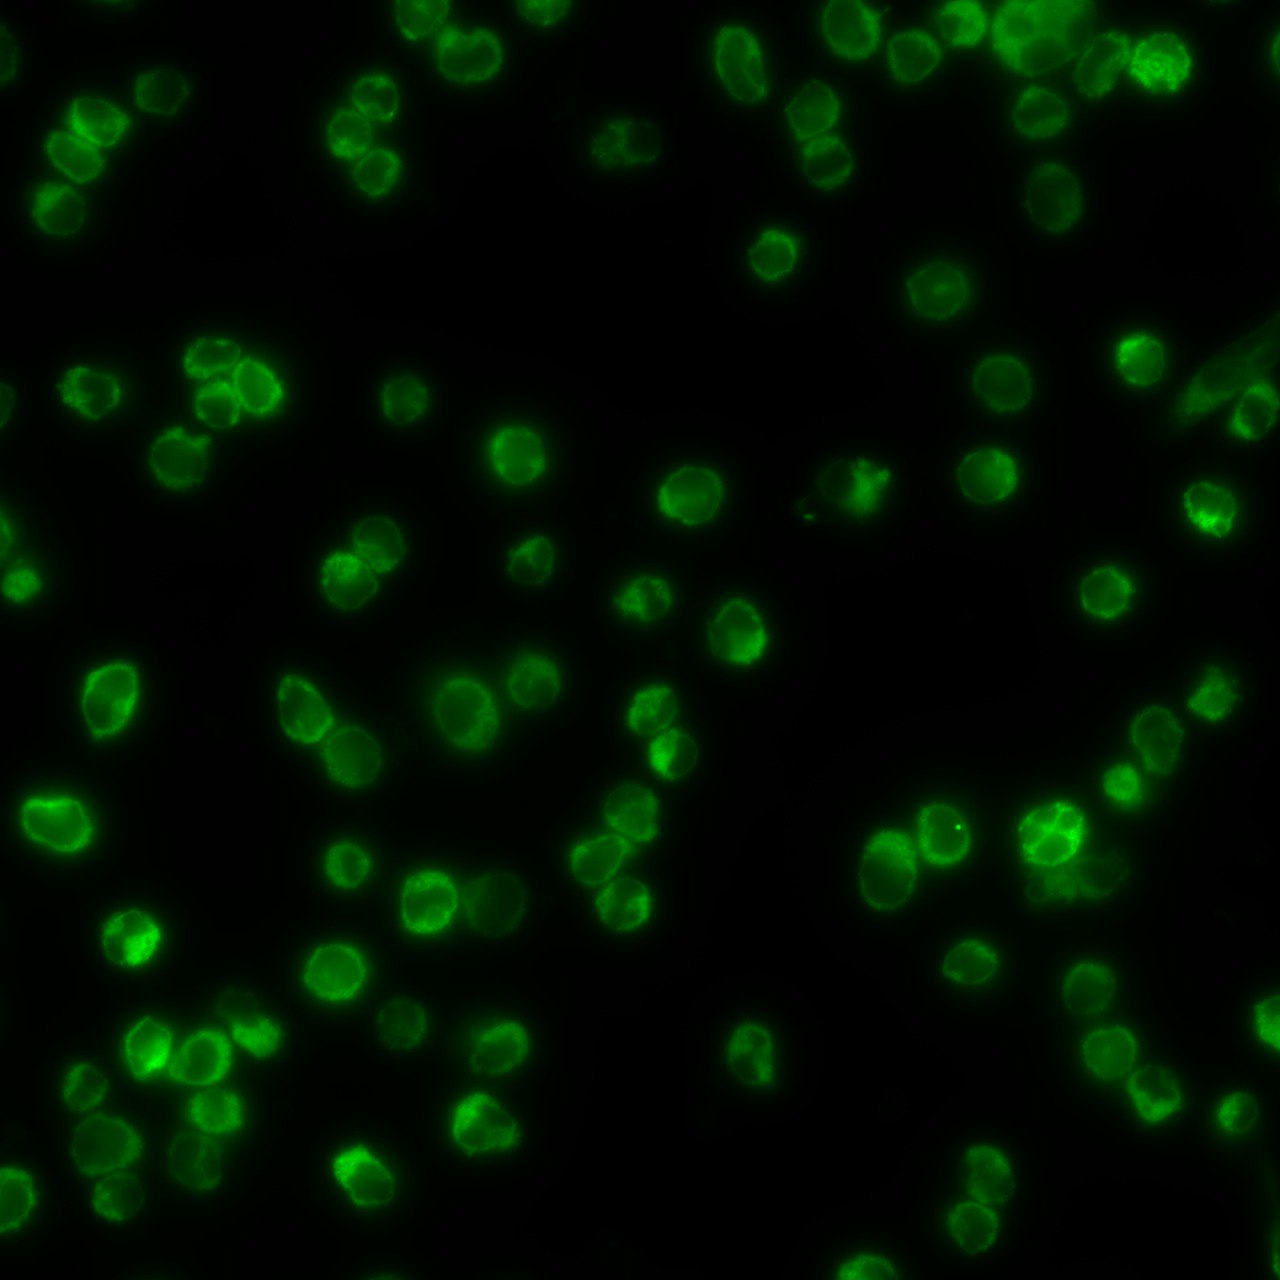
\includegraphics{bilder/ER/gt.jpg} & 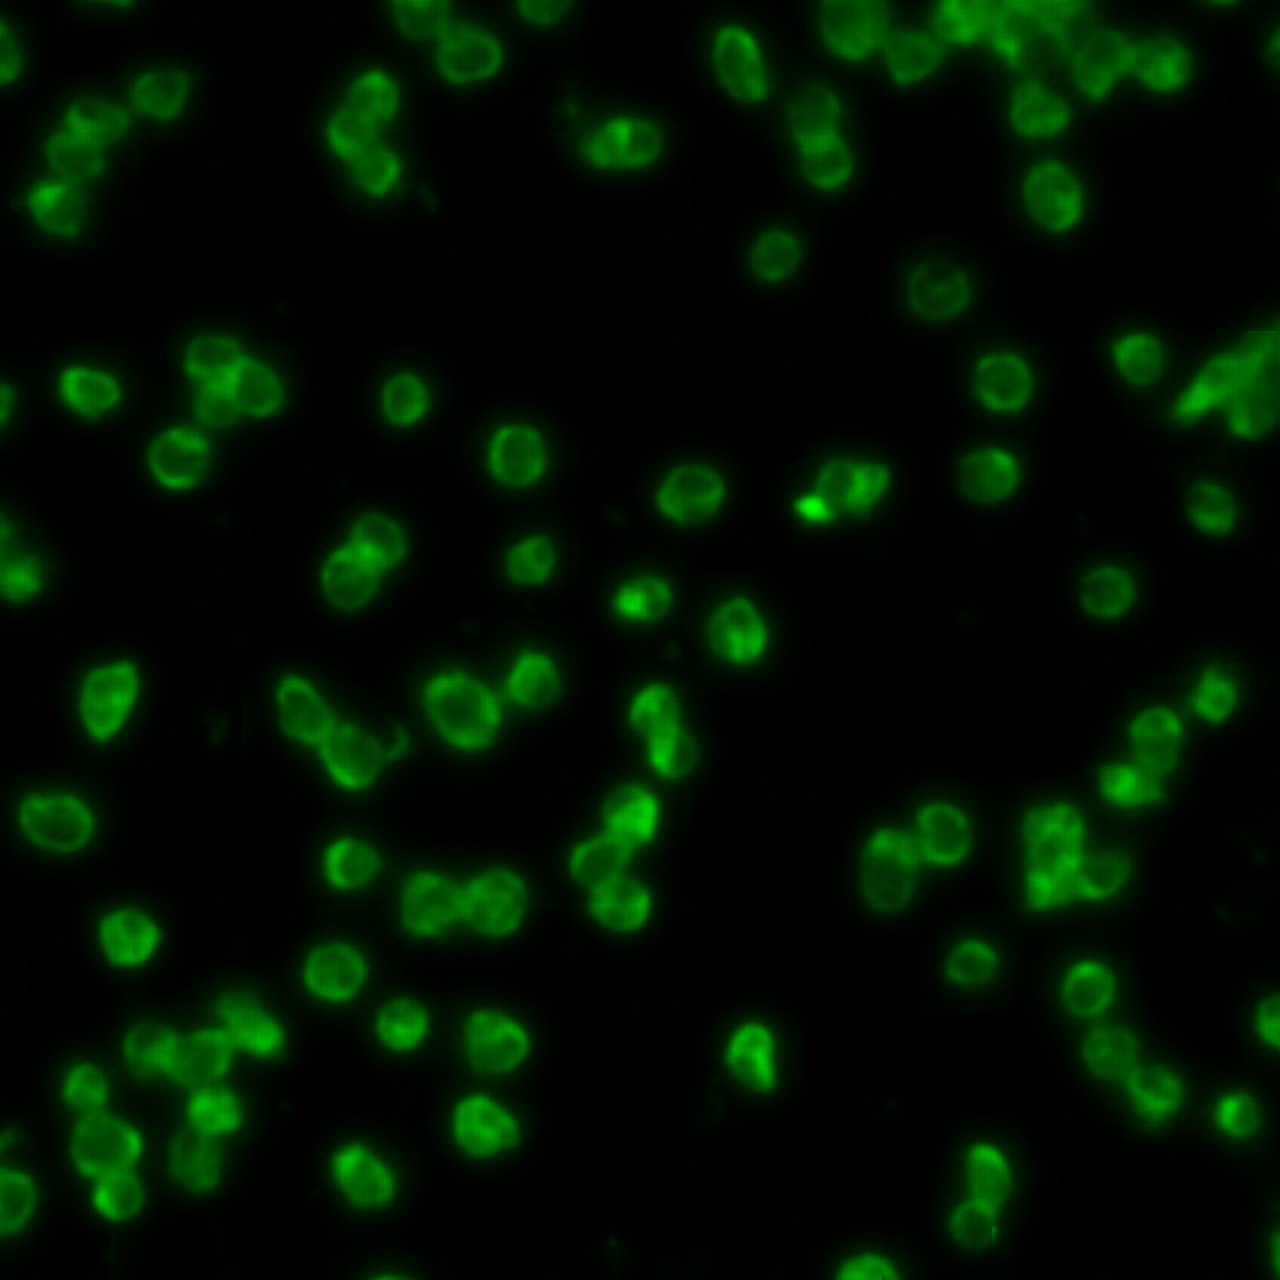
\includegraphics{bilder/ER/er.jpg} &
            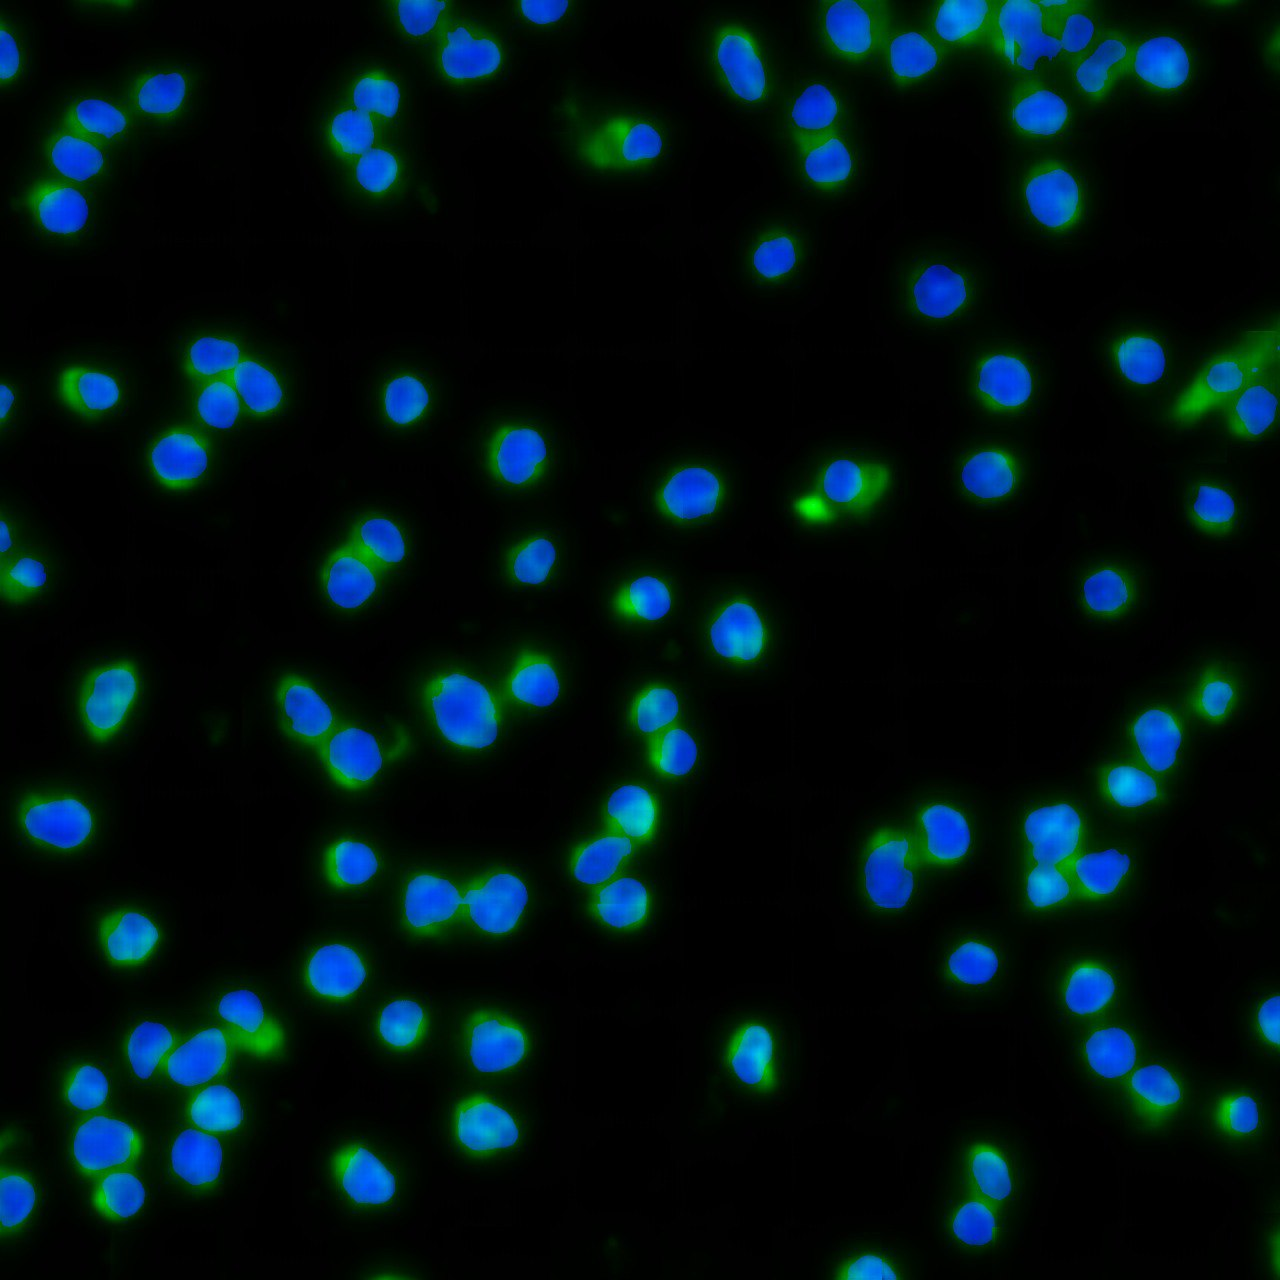
\includegraphics{bilder/ER/gt_nuclei.jpg}
        \end{tabularx}
    \caption{Combination of ER with nuclei prediction. Image (a) here is the original fluorescence image of ER, image (b) is the UNet prediction of ER and image (c) is the combination of predicted ER (green) with predicted nuclei (blue).}
    \label{fig:er-combined}
\end{figure}
    \subsubsection{Generalizability across phenotypes}
        TODO train the model on one phenotype and predict on the other, compare predictions (visually?) 
        postprocessing with metrics then?
        Add metrics
